\chapter{Impacto y M\'etricas}

EcoBrief mide el impacto a partir del flujo real del sistema. Las m\'etricas ambientales son estimaciones transparentes basadas en la reducci\'on de p\'aginas, art\'iculos y llamadas IA. A continuaci\'on se presentan los datos reales de la corrida del 15 de junio de 2026.

\section{Flujo del pipeline}

\begin{figure}[H]
\centering
\setlength{\fboxsep}{10pt}
\small
\begin{tabular}{c@{\hspace{0.5cm}}c@{\hspace{0.5cm}}c}
\fcolorbox{verde-ecobrief}{verde-ecobrief!5!white}{\parbox{2.8cm}{\centering\bfseries\Large 110\\[4pt] noticias\\[2pt] recolectadas\\[2pt] (100\%)}} &
\fcolorbox{gris-texto}{gris-claro}{\parbox{2.5cm}{\centering\small\bfseries 65\% descartadas\\[2pt] filtrado + dedup.\\[2pt] ranking + cach\'e}} &
\fcolorbox{verde-ecobrief}{verde-ecobrief!5!white}{\parbox{2.8cm}{\centering\bfseries\Large 39\\[4pt] briefs\\[2pt] generados\\[2pt] (35\%)}} \\
\end{tabular}
\vspace{6pt}

\fcolorbox{azul-profundo}{azul-profundo!5!white}{\parbox{0.85\textwidth}{\centering\bfseries 71 p\'aginas evitadas \quad| \quad 35.5\,min de lectura \quad| \quad 64.6\% de reducci\'on}}
\caption{Flujo del pipeline --- 15 de junio de 2026}
\end{figure}

\section{M\'etricas de la corrida}

\begin{table}[H]
\centering
\begin{tabular}{lrr}
\toprule
\textbf{M\'etrica} & \textbf{Valor} & \textbf{Porcentaje} \\
\midrule
Noticias recolectadas & 110 & 100\,\% \\
Art\'iculos \'utiles & 110 & 100\,\% \\
Art\'iculos \'unicos & 110 & 100\,\% \\
Briefs generados & 39 & 35\,\% \\
P\'aginas evitadas & 71 & 64.6\,\% \\
Minutos de lectura ahorrados & 35.5 & --- \\
\bottomrule
\end{tabular}
\caption{M\'etricas reales del 15 de junio de 2026}
\end{table}

\section{Panel de impacto}

\begin{figure}[H]
\centering
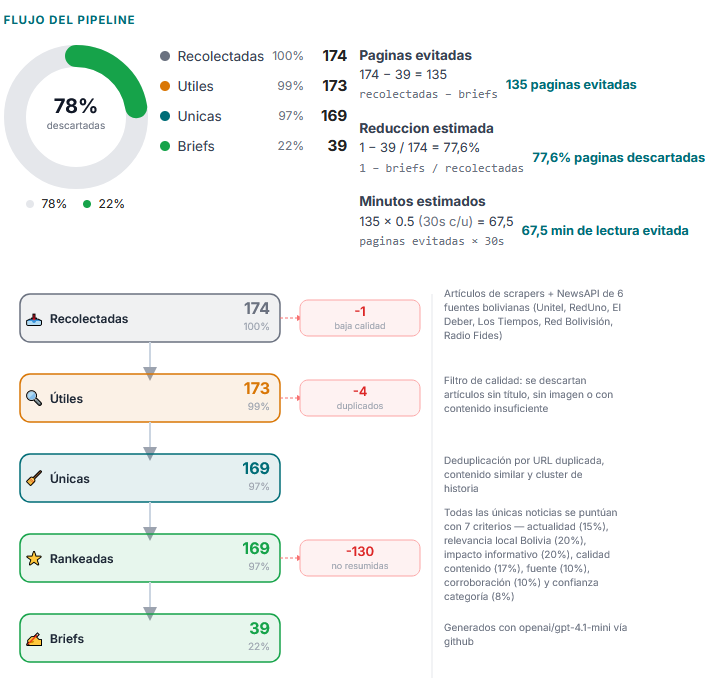
\includegraphics[width=\textwidth,keepaspectratio]{../images/metricas-15-junio-2026.png}
\caption{Panel de m\'etricas Green Tech -- 15 de junio de 2026}
\end{figure}

\section{F\'ormulas de impacto}

Las estimaciones se derivan de tres c\'alculos conservadores. Se define $R$ como el total de noticias recolectadas y $B$ como los briefs generados:

\paragraph{P\'aginas evitadas.} Diferencia entre lo recolectado y lo sintetizado:
\begin{equation}
P_{\text{evitadas}} = R - B = 110 - 39 = 71
\end{equation}

\paragraph{Tiempo de lectura ahorrado.} Estimando 30 segundos por p\'agina evitada:
\begin{equation}
M_{\text{ahorrados}} = P_{\text{evitadas}} \times 0.5 = 71 \times 0.5 = 35.5\text{ min}
\end{equation}

\paragraph{Tasa de reducci\'on del flujo.} Proporci\'on de contenido descartado respecto al total recolectado:
\begin{equation}
T_{\text{reducci\'on}} = 1 - \frac{B}{R} = 1 - \frac{39}{110} = 0.646 = 64.6\%
\end{equation}

\section{Nota metodol\'ogica}

Las m\'etricas ambientales son estimaciones operativas basadas en la reducci\'on de p\'aginas, art\'iculos y llamadas IA. No representan una medici\'on energ\'etica directa. EcoBrief es transparente sobre esta distinci\'on: reporta m\'etricas reales del pipeline y estimaciones derivadas, no mediciones de carbono o energ\'ia. Esta metodolog\'ia puede refinarse en fases posteriores del proyecto con herramientas especializadas de medici\'on.
